\documentclass[10pt]{beamer}

\usepackage[T1]{fontenc}
\usepackage[utf8]{inputenc}
\usepackage[lined,linesnumbered,commentsnumbered]{algorithm2e}
\usepackage{amsmath}
\usepackage{hyperref}
\usepackage{graphicx}

\useinnertheme{circles}
\useoutertheme{default}
\usecolortheme{orchid}
\setbeamertemplate{navigation symbols}{}



\begin{document}
  
  \title{Algorithms for social networks}
  \subtitle{PageRank}
  \author{Andreea Beica and Baptiste Lefebvre}
  \institute{\'{E}cole Normale Sup\'erieure\\Department of computer science}
  \date{27 january 2014}
  \maketitle

  
\begin{frame}
  \frametitle{Table of contents}
  \tableofcontents
\end{frame}


% Introduction %%%%%%%%%%%%%%%%%%%%%%%%%%%%%%%%%%%%%%%%%%%%%%%%%%%%%%%%%%%%%%%%%

\section{Introduction}

\begin{frame}
  \frametitle{Table of contents}
  \tableofcontents[currentsection]
\end{frame}

\begin{frame}
  \frametitle{Introduction}
  \textbf{PageRank} 
  \begin{itemize}
    \item Assess the importance of a web page based on its relationship with other pages
    \item Accurate description of user behaviour probability
    \item Objective measure of a web page's importance
  \end{itemize}
\end{frame}

\begin{frame}
  \frametitle{Introduction}
  \begin{figure}[h]
    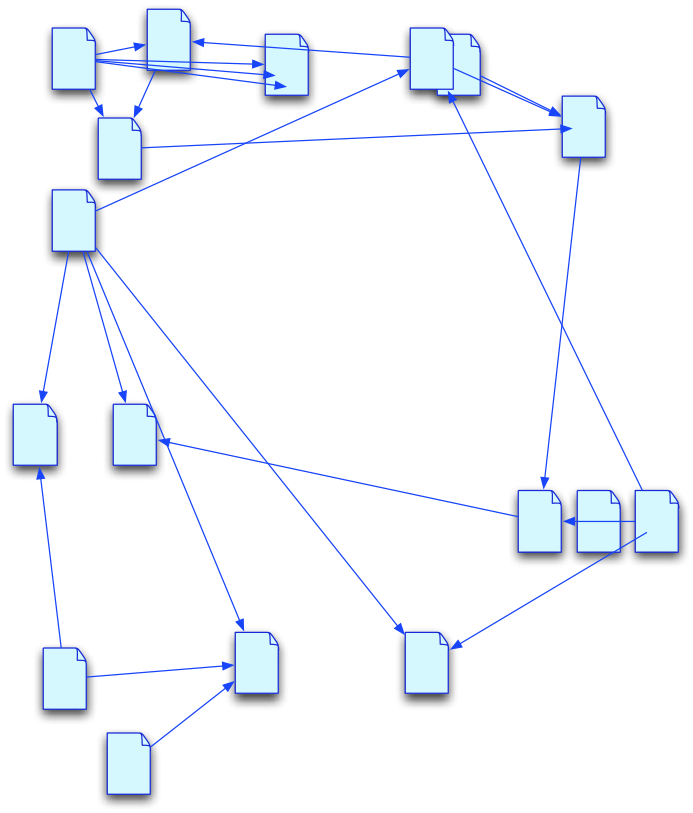
\includegraphics[width=0.5\textwidth]{webgraph.png}
    \caption{Network view of the web}
  \end{figure}
\end{frame}

\begin{frame}
  \frametitle{Introduction}
  \textbf{Text-based search engines}
  \begin{itemize}
    \item Rely primarily on information contained within the given page
    \item Titles with a high keyword density, search terms near the beginning of the document
    \item Easily manipulated, thus unreliable
  \end{itemize}
  \textbf{Our approach}
  \begin{itemize}
    \item PageRank + IR score
  \end{itemize}
\end{frame}


% PageRank %%%%%%%%%%%%%%%%%%%%%%%%%%%%%%%%%%%%%%%%%%%%%%%%%%%%%%%%%%%%%%%%%%%%%

\section{PageRank}

\begin{frame}
  \frametitle{Table of contents}
  \tableofcontents[currentsection]
\end{frame}

\begin{frame}
  \frametitle{Equation}
  $$ PageRank \left( i \right) = \frac{1 - d}{n} + d \sum\limits_{j \in M \left( i \right)} \frac{PageRank \left( j \right)}{L \left( j \right)} $$
\end{frame}

\begin{frame}
  \frametitle{Iterative method}
\IncMargin{1em}
\begin{algorithm}[H]
\SetKwInOut{Input}{Input}
\SetKwInOut{Output}{Output}
\BlankLine
\Indm
\Input{A webgraph $G$ with $n$ nodes}
\Output{An array $pr$ of size $n$}
\Indp
\BlankLine
\emph{// Initialization}\;
\For{$i \leftarrow 1$ \KwTo $n$}{
$pr'\left[i\right]\leftarrow\infty$\;
$pr\left[i\right]\leftarrow\frac{1}{n}$\;
}
\emph{// Iterations}\;
\While{$|pr-pr'|\geq\epsilon$}{
$pr' \leftarrow pr$\;
\For{$i \leftarrow 1$ \KwTo $n$}{
$pr\left[i\right]\leftarrow\frac{1-d}{N}+d\sum_{j\in M\left(i\right)}\frac{pr'[j]}{L\left(j\right)}$\;
}
}
\emph{// Renormalization}\;
$pr\leftarrow\frac{pr}{|pr|}$\;
\BlankLine
\end{algorithm}
\DecMargin{1em}
\end{frame}

\begin{frame}
  \frametitle{Algebraic method}
\IncMargin{1em}
\begin{algorithm}[H]
\SetKwInOut{Input}{Input}
\SetKwInOut{Output}{Output}
\BlankLine
\Indm
\Input{A adjacency matrix $A$ of a webgraph $G$ with $n$ nodes}
\Output{An array $pr$ of size $n$}
\Indp
\BlankLine
\emph{// Initialisation}\;
\For{$j \leftarrow 1$ \KwTo $n$}{
\If{$L\left(j\right) \neq 0$}{
\For{$i \leftarrow 1$ \KwTo $n$}{
$A\left[i\right]\left[j\right]\leftarrow \frac{A\left[i\right]\left[j\right]}{L\left(j\right)}$
}
}
}
\emph{Computation}\;
$pr\leftarrow \left(dA-I\right)^{-1}\frac{1-d}{n}O$
\BlankLine
\end{algorithm}
\DecMargin{1em}
\end{frame}

\begin{frame}
  \frametitle{Power method (1/2)}
  \IncMargin{1em}
  \begin{algorithm}[H]
    \SetKwData{Left}{left}\SetKwData{This}{this}\SetKwData{Up}{up}
    \SetKwFunction{Union}{Union}\SetKwFunction{FindCompress}{FindCompress}
    \SetKwInOut{Input}{Input}\SetKwInOut{Output}{Output}
    \BlankLine
    \Indm
    \Input{A webgraph $G$ with $n$ nodes}
    \Output{An array $pr$ of size $n$}
    \Indp
    \BlankLine
    \emph{// Initialization}\;
    \For{$i \leftarrow 1$ \KwTo $n$}{
    $pr'\left[i\right]\leftarrow\infty$\;
    $pr\left[i\right]\leftarrow\frac{1}{n}$\;
    }
  \end{algorithm}
  \DecMargin{1em}
\end{frame}

\begin{frame}
  \frametitle{Power Method (2/2)}
  \IncMargin{1em}
  \begin{algorithm}[H]
    \emph{// Iterations}\;
    \While{$|pr-pr'|\geq\epsilon$}{
    $pr' \leftarrow pr$\;
    \For{$i \leftarrow 1$ \KwTo $n$}{
    $pr\left[i\right]\leftarrow\frac{1-d}{N}+d\sum_{j\in M\left(i\right)}\frac{pr'[j]}{L\left(j\right)}$\;
    }
    \emph{// Renormalization}\;
    $s \leftarrow 0$\;
    \For{$i\leftarrow 1$ \KwTo $n$}{
    $s \leftarrow s + pr\left[i\right]$\;
    }
    \For{$i\leftarrow 1$ \KwTo $n$}{
    $pr\left[i\right] \leftarrow pr\left[i\right] + \frac{1-s}{n}$\;
    }
    }
    \BlankLine
  \end{algorithm}
  \DecMargin{1em}
\end{frame}


% System Architecture %%%%%%%%%%%%%%%%%%%%%%%%%%%%%%%%%%%%%%%%%%%%%%%%%%%%%%%%%%

\section{System architecture}

\begin{frame}
  \frametitle{Table of contents}
  \tableofcontents[currentsection]
\end{frame}

\begin{frame}
  \frametitle{System architecture}
  \begin{itemize}
    \item Simulate crawling and indexing the web (difficult)
    \item Instead: static HTML dumps of all Wikipedia pages for a chosen language
    \item All pages are crawled
    \item When "crawling" phase is done: graph of hyperlinks + inverted index
  \end{itemize}
\end{frame}

\begin{frame}
  \frametitle{System architecture}
  \textbf{Steps}
  \begin{enumerate}
    \item \textbf{Parsing}
      \begin{enumerate}
        \item Parse each page
        \item Construct \emph{invertedindex}
        \item Construct \emph{pointsTo}
      \end{enumerate}
    \item \textbf{Inverted index}
      \begin{enumerate}
        \item Used for quick lookup when a query is made
      \end{enumerate}
  \end{enumerate}
\end{frame}

\begin{frame}
  \frametitle{System architecture}
  \begin{figure}[h]
    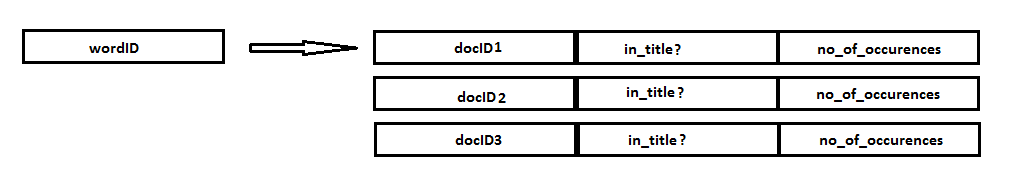
\includegraphics[width=0.8\textwidth]{index.png}
    \caption{Simplified inverted index}
  \end{figure}
\end{frame}

\begin{frame}
  \frametitle{IR score}
  \textbf{Information retrieval score}
  \begin{itemize}
    \item Determined by the emphasis and the weighted position of the specific terms in a document
    \item Used to compute the \emph{actual relevance}  of said document
    \item \emph{Actual relevance} of a page: $$IR\_score \times PageRank$$
    \item Our (simple) formula: $$nb\_occurences \times (in\_title + 1)$$
  \end{itemize}
\end{frame}

\begin{frame}
  \frametitle{Searching}
  For simplicity, we only refer to single word queries:
  \begin{enumerate}
    \item Look up query word in inverted index and retrieve corresponding doc list
    \item Compute IR score for each document
    \item Combine IR score and PageRank for each document in order to obtain final rank
    \item Sort documents and return first $k$
  \end{enumerate}
\end{frame}


% Results %%%%%%%%%%%%%%%%%%%%%%%%%%%%%%%%%%%%%%%%%%%%%%%%%%%%%%%%%%%%%%%%%%%%%%

\section{Results}

\begin{frame}
  \frametitle{Table of contents}
  \tableofcontents[currentsection]
\end{frame}

\begin{frame}
  \frametitle{Results for $\alpha = 0$}
  \begin{table}
    \begin{tabular}{ | c | c | c | c | l | }
      \hline
      Rank & IR Score & PR Score &  Score & Name \\ \hline
      1 & 8 & 0.000168 & 0.00134 & \href{http://rm.wikipedia.org/wiki/Categoria:(Stadi)_Germania}{Categoria: (Stadi) Germa...} \\ \hline
      2 & 8 & 0.000168 & 0.00134 & \href{http://rm.wikipedia.org/wiki/Germania}{Germania} \\ \hline
      3 & 6 & 0.000168 & 0.001005 & \href{http://rm.wikipedia.org/wiki/Rhaeti}{Rhaeti} \\ \hline
      4 & 6 & 0.000168 & 0.001005 & \href{http://rm.wikipedia.org/wiki/Categoria:Lieu_en_Germania}{Categoria: Lieu en Germa...} \\ \hline
      5 & 6 & 0.000168 & 0.001005 & \href{http://rm.wikipedia.org/wiki/Adolf_Hitler}{Adolf Hitler} \\ \hline
      6 & 6 & 0.000168 & 0.001005 & \href{http://rm.wikipedia.org/wiki/Categoria:Germania}{Categoria: Germania} \\ \hline
      7 & 3 & 0.000168 & 0.000503 & \href{http://rm.wikipedia.org/wiki/Renania-Palatinat}{Renania-Palatinat} \\ \hline
      8 & 3 & 0.000168 & 0.000503 & \href{http://rm.wikipedia.org/wiki/Lai_da_Constanza}{Lai da Constanza} \\ \hline
      9 & 3 & 0.000168 & 0.000503 & \href{http://rm.wikipedia.org/wiki/Hamburg}{Hamburg} \\ \hline
      10 & 3 & 0.000168 & 0.000503 & \href{http://rm.wikipedia.org/wiki/Hessen}{Hessen} \\ \hline
    \end{tabular}
    \caption{Results of the search engine for \emph{germania} with a damping factor of \emph{0.0} and the \emph{power method}}
    \label{table_d=0.0}
  \end{table}
\end{frame}

\begin{frame}
  \frametitle{Results for $\alpha = 0.85$}
  \begin{table}
    \begin{tabular}{ | c | c | c | c | l | }
      \hline
      Rank & IR Score & PR Score &  Score & Name \\ \hline
      1 & 1 & 0.043893 & 0.043893 & \href{http://rm.wikipedia.org/wiki/Spezial:Categories}{Spezial: Categories} \\ \hline
      2 & 8 & 0.001622 & 0.012974 & \href{http://rm.wikipedia.org/wiki/Germania}{Germania} \\ \hline
      3 & 3 & 0.004059 & 0.012178 & \href{http://rm.wikipedia.org/wiki/Svizra}{Svizra} \\ \hline
      4 & 2 & 0.001085 & 0.002169 & \href{http://rm.wikipedia.org/wiki/Categoria:Stadis_da_l'Europa}{Categoria: Stadis da l'Eur...} \\ \hline
      5 & 1 & 0.002023 & 0.002023 & \href{http://rm.wikipedia.org/wiki/Europa}{Europa} \\ \hline
      6 & 1 & 0.001513 & 0.001513 & \href{http://rm.wikipedia.org/wiki/Russia}{Russia} \\ \hline
      7 & 1 & 0.001439 & 0.001439 & \href{http://rm.wikipedia.org/wiki/Sinsheim}{Sinsheim} \\ \hline
      8 & 2 & 0.00062 & 0.00124 & \href{http://rm.wikipedia.org/wiki/Atletica}{Atletica} \\ \hline
      9 & 1 & 0.001191 & 0.001191 & \href{http://rm.wikipedia.org/wiki/Chantun_Argovia}{Chantun Argovia} \\ \hline
      10 & 3 & 0.000331 & 0.000994 & \href{http://rm.wikipedia.org/wiki/Organisaziun_da_las_Naziuns_unidas}{Organisaziun da las Naziu...} \\ \hline
    \end{tabular}
    \caption{Results of our search engine for \emph{germania} with a damping factor of \emph{0.85} and the \emph{power method}}
    \label{table_d=0.85}
  \end{table}
\end{frame}

\begin{frame}
  \frametitle{Results for $\alpha = 0.999999$}
  \begin{table}
    \begin{tabular}{ | c | c | c | c | l | }
      \hline
      Rank & IR Score & PR Score &  Score & Name \\ \hline
      1 & 1 & 0.057772 & 0.057772 & \href{http://rm.wikipedia.org/wiki/Spezial:Categories}{Spezial: Categories} \\ \hline
      2 & 8 & 0.001787 & 0.014297 & \href{http://rm.wikipedia.org/wiki/Germania}{Germania} \\ \hline
      3 & 3 & 0.004507 & 0.013521 & \href{http://rm.wikipedia.org/wiki/Svizra}{Svizra} \\ \hline
      4 & 1 & 0.003821 & 0.003821 & \href{http://rm.wikipedia.org/wiki/Europa}{Europa} \\ \hline
      5 & 2 & 0.001783 & 0.003565 & \href{http://rm.wikipedia.org/wiki/Categoria:Stadis_da_l'Europa_dfba}{Categoria: Stadis da l'Eur...} \\ \hline
      6 & 1 & 0.002766 & 0.002766 & \href{http://rm.wikipedia.org/wiki/Russia}{Russia} \\ \hline
      7 & 1 & 0.001333 & 0.001333 & \href{http://rm.wikipedia.org/wiki/Chantun_Argovia}{Chantun Argovia} \\ \hline
      8 & 1 & 0.001206 & 0.001206 & \href{http://rm.wikipedia.org/wiki/Frantscha}{Frantscha} \\ \hline
      9 & 1 & 0.00119 & 0.00119 & \href{http://rm.wikipedia.org/wiki/Alps}{Alps} \\ \hline
      10 & 1 & 0.001031 & 0.001031 & \href{http://rm.wikipedia.org/wiki/Liechtenstein}{Liechtenstein} \\ \hline
    \end{tabular}
    \caption{Results of our search engine for \emph{germania} with a damping factor of \emph{0.999999} and the \emph{power method}}
    \label{table_d=0.999999}
  \end{table}
\end{frame}

\begin{frame}
  \frametitle{Comparison with Google}
  \begin{table}
    \begin{tabular}{ | c | c | l | }
      \hline
      Rank & Google Rank & Name \\ \hline
      1 & - & \href{http://rm.wikipedia.org/wiki/Spezial:Categories}{Spezial: Categories} \\ \hline
      2 & 1 & \href{http://rm.wikipedia.org/wiki/Germania}{Germania} \\ \hline
      3 & 40 & \href{http://rm.wikipedia.org/wiki/Svizra}{Svizra} \\ \hline
      4 & 150 & \href{http://rm.wikipedia.org/wiki/Categoria:Stadis_da_l'Europa}{Categoria: Stadis da l'Europa} \\ \hline
      5 & 110 & \href{http://rm.wikipedia.org/wiki/Europa}{Europa} \\ \hline
      6 & 138 & \href{http://rm.wikipedia.org/wiki/Russia}{Russia} \\ \hline
      7 & 200+ & \href{http://rm.wikipedia.org/wiki/Sinsheim}{Sinsheim} \\ \hline
      8 & 200+& \href{http://rm.wikipedia.org/wiki/Atletica}{Atletica} \\ \hline
      9 & 200+ & \href{http://rm.wikipedia.org/wiki/Chantun_Argovia}{Chantun Argovia} \\ \hline
      10 & 115 & \href{http://rm.wikipedia.org/wiki/Organisaziun_da_las_Naziuns_unidas}{Organisaziun da las Naziuns unidas} \\ \hline
    \end{tabular}
    \caption{Comparison with Google results ( \emph{rm.wikipedia.org} domain restriction) for \emph{germania} with a damping factor of \emph{0.85}}
    \label{table_comparison}
  \end{table}
\end{frame}

\begin{frame}
  \frametitle{Results on a larger dataset}
  \begin{table}
    \begin{tabular}{ | c | c | c | c | l | }
      \hline
      Rank & IR Score & PR Score &  Score & Name \\ \hline
      1 & 198 & 0,002858 & 0,56581 & \href{http://af.wikipedia.org/wiki/Duitsland}{Duitsland} \\ \hline
      2 & 19 & 0,003674 & 0,0698 & \href{http://af.wikipedia.org/wiki/Frankryk}{Frankryk} \\ \hline
      3 & 46 & 0,000316 & 0,014535 & \href{http://af.wikipedia.org/wiki/Duitse_Demokratiese_Republiek}{Duitse Demokratiese Repu...} \\ \hline
      4 & 21 & 0,000468 & 0,009829 & \href{http://af.wikipedia.org/wiki/Berlyn}{Berlyn} \\ \hline
      5 & 6 & 0,001097 & 0,006584 & \href{http://af.wikipedia.org/wiki/België}{Belgi\"{e}} \\ \hline
      6 & 26 & 0,000201 & 0,00523 & \href{http://af.wikipedia.org/wiki/Frankfurt_am_Main}{Frankfurt am Main} \\ \hline
      7 & 5 & 0,001024 & 0,00512 & \href{http://af.wikipedia.org/wiki/Duits}{Duits} \\ \hline
      8 & 8 & 0,000632 & 0,00506 & \href{http://af.wikipedia.org/wiki/Denemarke}{Denemarke} \\ \hline
      9 & 3 & 0,001148 & 0,003444 & \href{http://af.wikipedia.org/wiki/Frans}{Frans} \\ \hline
      10 & 2 & 0,001702 & 0,003405 & \href{http://af.wikipedia.org/wiki/Afrikaans}{Afrikaans} \\ \hline
    \end{tabular}
    \caption{Results of our search engine for \emph{duitsland} with a damping factor of \emph{0.85} and the \emph{power method}}
    \label{table_larger}
  \end{table}
\end{frame}


% Conclusion %%%%%%%%%%%%%%%%%%%%%%%%%%%%%%%%%%%%%%%%%%%%%%%%%%%%%%%%%%%%%%%%%%%

\section{Conclusions}

\begin{frame}
  \frametitle{Table of contents}
  \tableofcontents[currentsection]
\end{frame}

\begin{frame}
  \frametitle{Conclusions}
  \begin{itemize}
    \item Small functional search engine
    \item Significant number of pages ($15000$ in the Afrikaans case)
    \item Significant size of hyperlink graph
  \end{itemize}
\end{frame}

\begin{frame}
  \frametitle{Error sources}
  \begin{itemize}
    \item Data fetching
    \item Outdated databases
    \item Memory limitations
    \item Simple models for the inverted index and the IR score
  \end{itemize}
\end{frame}


%%%%%%%%%%%%%%%%%%%%%%%%%%%%%%%%%%%%%%%%%%%%%%%%%%%%%%%%%%%%%%%%%%%%%%%%%%%%%%%%

\section{}

\begin{frame}
  \frametitle{Thanks}
  \begin{center}
    \huge{Thanks !}
  \end{center}
\end{frame}

\begin{frame}
  \frametitle{References (1/3)}
  \begin{thebibliography}{1}
    \bibitem{Witten94}
      I. Witten, A. Moffat, and T. Bell\\
      \textbf{Managing Gigabytes: Compressing and Indexing Documents and Images}\\
      \emph{Van Nostrand Reinhold, 1994}
    \bibitem{Brin98}
      S. Brin, and L. Page\\
      \textbf{The Anatomy of a Large-Scale Hypertextual Web Search Engine}\\
      \emph{Computer Networks and ISDN Systems, 1998}
    \bibitem{Cho98}
      J. Cho, H. Garcia-Molina, and L. Page\\
      \textbf{Efficient Crawling Through URL Ordering}\\
      \emph{7th International Web Conference, 1998}
  \end{thebibliography}
\end{frame}

\begin{frame}
  \frametitle{References (2/3)}
  \begin{thebibliography}{1}
    \bibitem{Page98}
      L. Page, S. Brin, R. Motwani, and T. Winograd\\
      \textbf{The PageRank Citation Ranking: Bringing Order to the Web}\\
      \emph{Technical Report, 1999}
    	\bibitem{Haveliwala99}
    	  T. Haveliwala\\
    	  \textbf{Efficient Computation of PageRank}\\
    	  \emph{Technical Report, 1999}
    	\bibitem{Richardson02}
    	  M. Richardson, and P. Domingos\\
    	  \textbf{The Intelligent Surfer: Probabilistic Combination of Link and Content Information in PageRank}\\
    	  \emph{Advances in Neural Information Processing Systems 14, 2002}
  \end{thebibliography}
\end{frame}

\begin{frame}
  \frametitle{References (3/3)}
  \begin{thebibliography}{1}
    \bibitem{Haveliwala03}
      T. Haveliwala, S. Kamvar, and G. Jeh\\
    	  \textbf{An Analytical Comparison of Approaches to Personalizing PageRank}\\
    	  \emph{Technical Report, 2003}
    	\bibitem{Berkhin05}
    	  P. Berkhin\\
      \textbf{A Survey on PageRank Computing}\\
    	  \emph{Internet Mathematics, 2005}
    \bibitem{Bianchini05}
      M. Bianchini, M. Gori, and F. Scarselli\\
      \textbf{Inside PageRank}\\
      \emph{Transactions on Internet Technologies, 2005}
  \end{thebibliography}
\end{frame}

\end{document}